\def\stitle{\theexercise\ - Programmentwicklung}
\section{\stitle}
\begin{frame}%
  \frametitle{\stitle}%
\tableofcontents[current]
\end{frame}


\begin{frame}%
  \frametitle{\stitle}%

\begin{itemize}
\item Wozu dient der Java-Compiler, wozu der Java-Interpreter?
\item Erläutern Sie die Aussage \glqq Java ist plattformunabhängig\grqq.
\end{itemize}

\end{frame}


\begin{frame}[t]%
  \frametitle{\stitle\ Fortsetzung}%
\centering

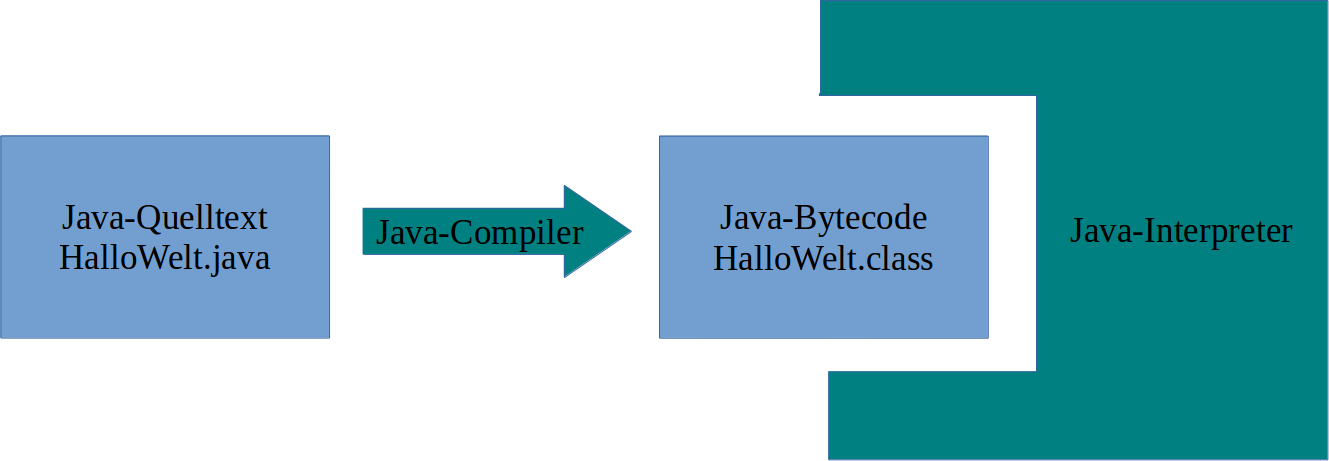
\includegraphics[width=0.6\textwidth]{grundl-java/Java-Kompiler}\\[2em]

\includegraphics[width=0.6\textwidth]{grundl-java/C++-Kompiler}

\begin{itemize}
 \item Java-Bytecode ist plattformunabhängig und kann vom Java-Interpreter auf jedem System ausgeführt werden.
 \item C++ Programme können direkt vom Betriebssystem ausgeführt werden, wenn sie für dieses kompiliert wurden.
\end{itemize}

\end{frame}
